\documentclass{article}

\usepackage{minted}
\usepackage{amsmath, amsthm}
\usepackage{amssymb}
\usepackage{listings}
\usepackage[svgnames]{xcolor}
\usepackage{tikz}
\usepackage{array}
\usepackage{graphicx}
\usepackage[backend=biber, maxbibnames=9]{biblatex}
\usepackage{algpseudocode}
\usepackage{algorithm}
\usepackage{mathtools}
\usepackage[rightcaption]{sidecap}
\usepackage{subcaption}
\usepackage{hyperref}

\graphicspath{ {./images/} }

\addbibresource{report.bib}

\title{Conjure: A Computer Vision Controller Using Hand Gestures}
\author{Anthony Hunt}

\begin{document}
\maketitle

\section{Introduction}
Over the last 20 years, extraordinary progress in image processing and CNNs have brought about revolutionary methods of interacting with the world. From self-driving cars to early cancer detection, computer vision has become integral to interactions with technology and our environments. The usefulness of such software is self-evident in its pervasiveness within smartphones and personal computing; home buttons have been replaced with retina scanners and facial recognition, VR headsets no longer need dedicated controllers, and any device can read handwritten text directly from a photo.

In the gradual rollout of virtual hands-free computing, gesture-based interactions serve as a natural and intuitive platform for communicating with computers. This project, named Conjure, aims to take gesture-based interactions one step further by providing human-computer interactions with only a camera and hand recognition software. However, unlike the Xbox Kinect or Apple Vision Pro headset, which make use of depth sensors in addition to regular cameras, we attempt to use only a standard camera. Of course, the use case of Conjure is far simpler than that of VR headsets or game consoles, since the target platform this program is user-facing laptop webcams. We can further assume that most people interact with webcams in an egocentric view, that is, facing the camera with one prominent subject and a mostly static background.

The rest of this report will outline the features of Conjure along with instructions to get started, the model architectures explored and used within the program, some key results, and difficulties throughout the project.

\section{Usage}
To get started, clone the \href{https://github.com/Ant13731/conjure}{GitHub repository} and download all dependencies through \texttt{pip install -r requirements.txt}. Ensure the computer's webcam is plugged in and working, then run \texttt{python main.py}. Note that this project was tested with Python 3.12 on a Windows machine.

Upon startup, a GUI containing settings and other options should appear similar to Figure~\ref{fig:config}
\sidecaptionvpos{figure}{c}
\begin{SCfigure}[2][h]
    \centering
    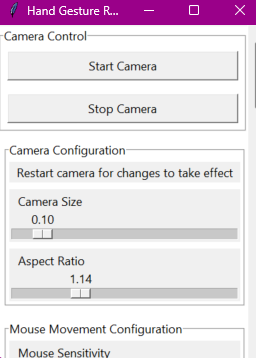
\includegraphics[height=4cm]{config.png}
    \caption{Startup configuration UI. Click Start/Stop Camera to activate the virtual controller.}
    \label{fig:config}
\end{SCfigure}

The main interactions of Conjure are as follows, with coinciding images in Figure~\ref{fig:gestures}:
% TODO add in images of gestures, also add to README
\begin{itemize}
    \item Hand movement in the camera's 2D projection of 3D space coincides with mouse movement across a computer's monitor. For fine-grained movements and other interactions, Conjure creates a deadzone at the center of the screen, where all hand movements are ignored. Then, as a hand moves out of the deadzone toward the borders of the screen, the mouse will move with increasing velocity in the hand's general direction.
    \item Simulating a left click can be done by making an ``OK'' gesture towards the camera. This gesture is closest to the natural pinch gestures of VR headsets while being freely available in many datasets \cite{Alexander_2024, nuzhdin2024hagridv21mimagesstatic, zimmermann2017learningestimate3dhand, gesture_recognizer}.
    \item A right click conversely uses a ``peace'' sign, with the index and middle fingers extended and pointing away from each other.
    \item A click-and-hold motion makes use of a closing fist gesture. As long as the fist remains closed, the mouse will continue holding down the button. Moving around the camera space while maintaining a closed fist allows for drag-and-drop behaviours.
    \item Exiting the program is done with a ``reverse-stop'' motion, where the hand is fully extended, fingers close to one another, and the user's palm is facing away from the camera.
    \item Scrolling coincides with a two-finger-raised gesture, with up and down behaviour following the palm's direction - up when facing towards and down when facing away from the camera respectively. During testing, I found that scrolling behaviours worked best if it was only used in a specific area of the screen. Thus, this gesture only works within the scroll zone (by default, this is the right side of the mouse deadzone).
\end{itemize}

All gesture-specific actions may be changed with the GUI configuration, made in Tkinter. Other options, like movement sensitivity, deadzone sizes, etc., are also configurable through the UI.

\begin{figure}
    \centering
    \begin{subfigure}[T]{0.76\textwidth}
        \centering
        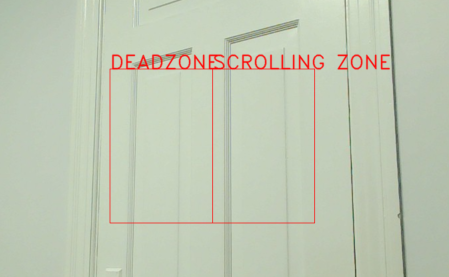
\includegraphics[width=.8\linewidth]{deadzone.png}
        \caption{The left deadzone prevents hand movement within that area from controlling the mouse. Any gestures will work in this area. The right scroll zone prevents mouse movement but enables scrolling movement. Pointing two fingers up when the index finger is within this zone will perform a scroll-up action.}
    \end{subfigure}
    \begin{subfigure}[T]{0.3\textwidth}
        \centering
        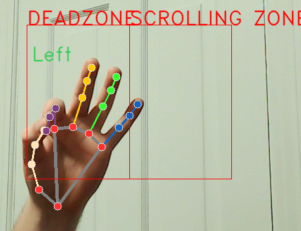
\includegraphics[width=.8\linewidth]{ok.png}
        \caption{OK symbol for left click.}
    \end{subfigure}\hfill
    \begin{subfigure}[T]{0.3\textwidth}
        \centering
        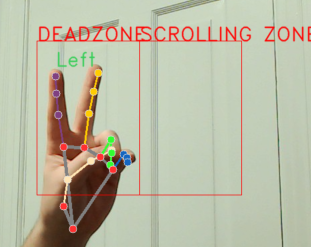
\includegraphics[width=.8\linewidth]{peace.png}
        \caption{Peace symbol for right click.}
    \end{subfigure}\hfill
    \begin{subfigure}[T]{0.3\textwidth}
        \centering
        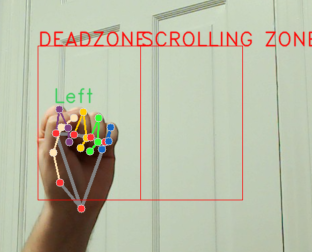
\includegraphics[width=.8\linewidth]{fist.png}
        \caption{Clenching a hand will mirror click-and-hold behaviour.}
    \end{subfigure}
    \begin{subfigure}[T]{0.3\textwidth}
        \centering
        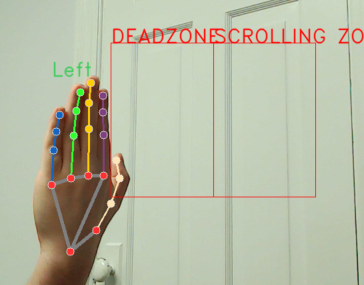
\includegraphics[width=.8\linewidth]{stop_inverted.png}
        \caption{A stop symbol with the palm facing away from the camera will exit the camera control program.}
    \end{subfigure}\hfill
    \begin{subfigure}[T]{0.3\textwidth}
        \centering
        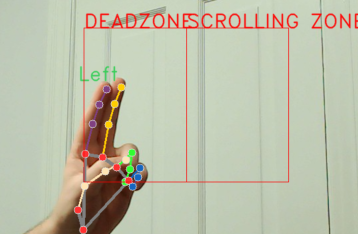
\includegraphics[width=.8\linewidth]{two_up.png}
        \caption{Two fingers pointing up will scroll up (only in the right side scroll zone).}
    \end{subfigure}\hfill
    \begin{subfigure}[T]{0.3\textwidth}
        \centering
        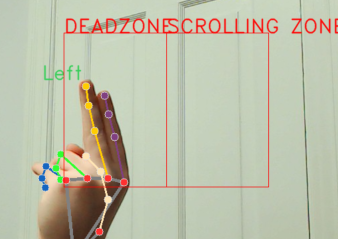
\includegraphics[width=.8\linewidth]{two_up_inverted.png}
        \caption{Showing the back of the scroll-up gesture will scroll down (only in the right side scroll zone).}
    \end{subfigure}
    \caption{A collection of gestures described in section 2.}
    \label{fig:gestures}
\end{figure}

% likely will have the conjure folder zipped in avenue
% need to unzip, install requirements, run, also show how to train

\section{Model and Method}
When looking for similar projects in hand recognition and gesture detection, Google's Mediapipe suite of models \cite{gesture_recognizer} is among the first and most performant entries. A sizeable portion of this project uses the Mediapipe hand landmarking model to track hands in 3D space, along with a fine-tuned version of their gesture classification model retrained on the HaGRID dataset \cite{Alexander_2024}. Mediapipe also provides convenient functions for projecting hand skeletons on the webcam's video feed (as seen in Figure~\ref{fig:gestures}).

Originally, I had planned to create my own CNN model from scratch (as seen in the \texttt{model/old\_attempts} folder), training on the Rendered Handpose Dataset \cite{zimmermann2017learningestimate3dhand}. This process would have included a CNN landmarking model to project key hand joints in 2D space alongside a second fully-connected network to classify the points into useful gestures. However, a combination of hardware limitations, data preprocessing, and overly simple model architecture failed to capture the objective hand location data, resulting in extreme overfitting when compared with a validation set.

After spending a few days investigating the poor performance of my own model and researching CNNs for object detection, I came across an old Mediapipe blog post \cite{mediapipeLegacyHands} detailing the data pipeline for the entire hand recognition process. With a bit of simplification, the general process of classification is as follows:
\begin{enumerate}
    \item A Single Shot Detector (SSD) model \cite{Liu_2016} is first used to recognize the bounding boxes of palms within the image. Generally, SSD models are specialized CNNs without final fully-connected layers that make use of bounding box anchors to simultaneously predict the location and classification of objects. Training data passed to this model must be prepared with hundreds of anchor points that enable the model to pinpoint the exact contributions of anchors to the object's location. Although data preparation is intense, SSDs generally perform far better and more efficiently than CNN counterparts, contributing to the real-time nature of livestream hand detection.
    \item After the general location of a hand has been processed through the SSD, the original image is cropped to relevant regions and passed through a regular CNN. By virtually eliminating all non-hand objects from the image, this model can focus on finding landmarks within the hand, rather than finding the hand within an entire image. Key points can then be converted back into the original image's coordinates and prepared for classification. The current version of the gesture recognizer \cite{gesture_recognizer} provides further computational benefits in tracking hand motion over multiple frames when set to ``video'' or ``livestream'' mode.
    \item From the relative locations of landmarks, Mediapipe uses a simple fully-connected model to finally classify the gesture.
\end{enumerate}

Although I have some experience making CNNs in an academic setting, creating a full SSD model from scratch felt far beyond the scope of this project, especially with limited time, processing power, and overall lack of familiarity in manipulating image data. An alternative scheme wherein a pre-made SSD model is used in conjunction with custom models for stages 2 and 3 of the pipeline would have been manageable, however there were understandably few resources on the topic. Mediapipe only offers end-to-end complete models through their API and GitHub, and the only similar project \cite{Dibia2017} contained several dependency-related issues between tensorflow v1 and v2, preventing access to the weights in a usable form. Because Mediapipe offered a complete, highly performant and customizable classification pipeline, I opted to use their API and architecture, only finetuning hyperparameters and providing training data for the 3rd-stage model.

Therefore, instead of creating deep learning models from source, this project takes a more application-focused approach to machine learning. While imperfect, the live video feed, GUI, and extensive configuration all attempt to make the project more usable for its end goal: providing a virtual trackpad with only camera input.

% model architecture: 3 of them, 1. SSD, 2. Regression CNN, 3. Classification CNN

\section{Results}
The retrained stage 3 classifier model performed well fairly quickly, only requiring 20 iterations of training on a 30,000 image dataset \cite{Alexander_2024} to achieve 90\% accuracy. The classifier model contained 2 relatively small units of fully connected layers, performing best with a learning rate of 0.005 and dropout rate of 0.1. Steady improvements in both training and validation over 50 epochs can be seen in Figure~\ref{fig:graphs}.

\begin{figure}[h]
    \centering
    \begin{subfigure}[T]{0.5\textwidth}
        \centering
        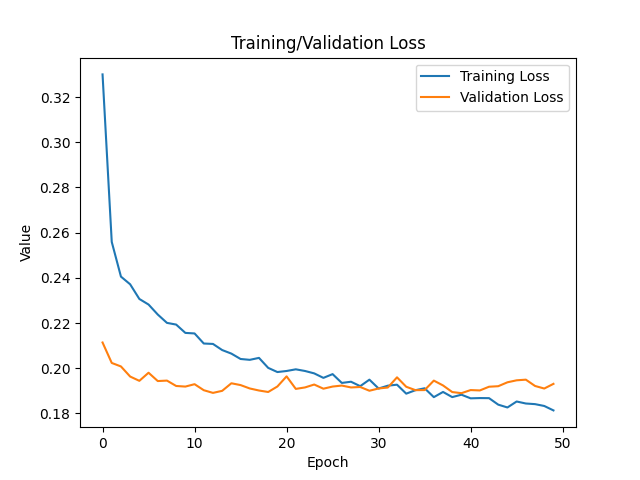
\includegraphics[width=\linewidth]{loss_graph.png}
    \end{subfigure}\hfill
    \begin{subfigure}[T]{0.5\textwidth}
        \centering
        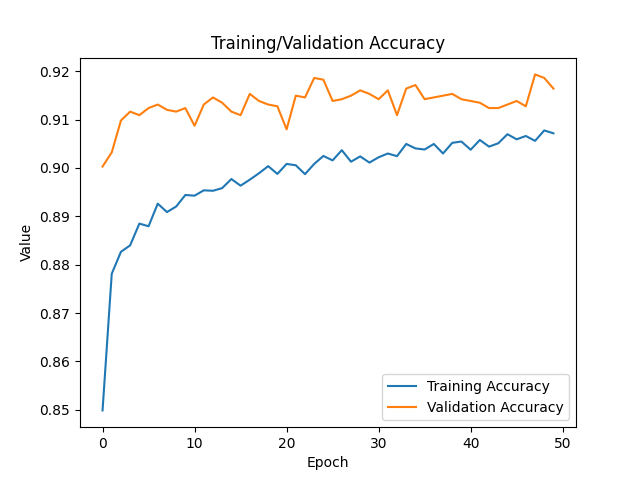
\includegraphics[width=\linewidth]{accuracy_graph.png}
    \end{subfigure}
    \caption{Results of training and validation of the stage 3 classifier model on 30,000 samples of the HaGRID \cite{Alexander_2024} dataset}
    \label{fig:graphs}
\end{figure}

On the interaction side of Conjure, the application is separated into two parts. First, the main GUI controls and updates all configuration changes in real-time. Sliders and dropdown menus are provided to change deadzone properties, gestures, and other similar settings. Then, two buttons control the camera livestream component, which performs classification predictions and gesture-to-action mouse movement.

In the initial stages of testing, the classifier model, although highly accurate for still images, sometimes had trouble identifying frames involving rapid swaps between two similar gestures. For example, a ``peace'' sign may be mistaken for a ``two-fingers-up'' gesture when transitioning from ``peace'' to a closed fist, and vice versa. This could introduce undesired scrolling or clicking behaviours, reducing the reliability of the computer control. However, requiring around 3 consecutive frames of input before performing an action seemed to resolve a large amount of such cases. Explicit landmark calculations for identifying the front/back of hands also helped to resolve differences in, for example, identifying a left-hand's stop versus a right-hand's inverted stop gestures.


% First tried CNN, show loss curve
% TOMORROW: Use https://github.com/victordibia/handtracking as a pretrained model to just detect the bounding boxes of hands. then follow the google guide, crop photo (scale image up to original first model size, pad the difference to accommodate diff aspect ratios), predict coordinates, then pass coords to a fully connected NN for classification.
% Had a plan, not enough time to execute
% Final project, using pretrained 1 and 2 models, custom data passed to classifier model, show loss curve for classifier model
\section{Conclusion}

While CNNs are a relatively old concept in the fast-paced field of machine learning, modern interpretations on convolutions may continue to increase the usefulness and viability of computer vision in ever-critical applications. Among the burst of popularity of generative text-based models and image creation, computer vision in particular shows great promise in shaping a more accessible and convenient future. For instance, projects like this one could be trivially extended with gestures to enable speech-to-text input or simplified video game controls for those with limited finger mobility, without the need for dedicated hardware. Although the process of making Conjure did not turn out quite as expected, the final product is more than satisfiable in providing users with a proof-of-concept virtual trackpad interface.



\pagebreak
\nocite{*} % keeps all references, even those not referred to
\printbibliography %Prints bibliography
\end{document}

